%
% File acl2015.tex
%
% Contact: car@ir.hit.edu.cn, gdzhou@suda.edu.cn
%%
%% Based on the style files for ACL-2014, which were, in turn,
%% Based on the style files for ACL-2013, which were, in turn,
%% Based on the style files for ACL-2012, which were, in turn,
%% based on the style files for ACL-2011, which were, in turn, 
%% based on the style files for ACL-2010, which were, in turn, 
%% based on the style files for ACL-IJCNLP-2009, which were, in turn,
%% based on the style files for EACL-2009 and IJCNLP-2008...

%% Based on the style files for EACL 2006 by 
%%e.agirre@ehu.es or Sergi.Balari@uab.es
%% and that of ACL 08 by Joakim Nivre and Noah Smith

\documentclass[journal,onecolumn, 12pt]{article}
\usepackage[a4paper, margin=1in]{geometry}
%%\usepackage{acl2015}
\usepackage{times}
\usepackage{url}
\usepackage{latexsym}
\usepackage{graphicx}
\usepackage{fancyvrb}
\usepackage{amsmath}
\usepackage[font=small,skip=1pt]{caption}
\usepackage{subcaption}
\graphicspath{ {./images/} }

%\setlength\titlebox{5cm}

% You can expand the titlebox if you need extra space
% to show all the authors. Please do not make the titlebox
% smaller than 5cm (the original size); we will check this
% in the camera-ready version and ask you to change it back.
\pagestyle{plain}

\title{Relaxation and Memory \\
\large An Experimental Study on State of Mind and Memory Recall \\
\medium Summer 2020 - W241 Final Project}

\author{
\\
{Chitra S. Agastya,  \tt chitra.agastya@berkeley.edu} \\
{James Gao, \tt jamesygao55@berkeley.edu}\\
{Wenqi Liu, \tt wenqiliu@berkeley.edu}\\
\\
}

\begin{document}

\setlength{\belowcaptionskip}{-10pt}
\setlength{\abovedisplayskip}{-10pt}
\setlength{\belowdisplayskip}{-10pt}

\maketitle
\begin{abstract}

\noindent
Whether one is managing a job, a business, studies or home life, one is likely to benefit from memory recall and focus. Distractions caused by day to day activities like excessive screen time,  stressful multitasking, inadequate sleep, poor sleeping habits etc. cause information overload in our brains and are likely to compromise our ability to stay focused and be productive to our best potential. Does a relaxed mind help one to remember information better? In this project, we attempt to study the impact the state of our mind may have on memory recall by running a simple intervention based experiment that gives people either a calming or a stressful audio treatment and then looks at their short term memory recall scores from on a simple math game.

\end{abstract}

\section{Background}

We are in an information and new media age where our brain is constantly exposed to information from a plethora of media and digital devices. People have become more reliant on technology, whose power of retention is far more, to stand in for human memories. With this barrage of information, how might one cope with making a mental note of day to day facts? \\

\noindent
Is a calmer mind better suited for cognitive awareness? The answer to this question, substantiated with empirical data, could potentially help us tackle the problem with memory recall. It could help us create learning plans and therapies for people with learning disabilities and some types of dementia and could aid students with attention deficiencies who are unable to adequately focus on learning activities. A Reuters science news article published in March 2010\footnote {“Scientists find how relaxed minds remember better” Reuters Science News, March 24 2010,
https://www.reuters.com/article/us-memory-brainwaves/scientists-find-how-relaxed-minds-remember-better-idUSTRE62N4VJ20100324
} discussed a neuroscience theory that robust, longer lasting memories are likely to be formed when the mind is relaxed. The neuroscientists suggest that when the brain is relaxed, the memory related neurons fire in synchronization and when these memory related neurons are well coordinated, memories are stronger. Understanding the causal relationship between the state of our mind and the ability to remember could be a crucial step in counterbalancing the brain fog we are subjected to in this age of information overload. 


\section{Research Question}

The primary research question we are trying to answer here is: does relaxation of ones mind make one to remember better? There are several Yoga and mindful breathing workshops that try to tackle the problem of mental stress. One of the benefits of such workshops is said to be the calming impact on the mind and the improvement to memory recall. \\

\section{Hypothesis}
Motivated by the general principles of yoga and mindful breathing, our primary hypothesis is that a relaxed mind can remember information better. In addition to our primary research question, we are also interested in seeing if factors like gender, time of the day and formal music training have an effect on memory recall. We analyze the experimental data in the light of these control variables. to see if they have an effect on memory recall. We additionally hypothesize that: 1. people with significant music training are better at memory recall because their minds are formally trained to recall music. 2. memory recall may be higher when a person is relatively less busier during the day, such as closer to office/school ending hours. We believe that gender might not impact memory recall.

\section {Experiment}

\subsection {Overview}
To test our hypothesis that addresses the research question at hand, we design a difference-in-differences experiment with an intervention that would supposedly induce some form of mental relaxation. We use a simple Math game of Digit Span\footnote {“How Many Numbers Can You Remember?” Science Buddies, 28 July 2017, https://www.sciencebuddies.org/science-fair-projects/project-ideas/HumBehp020/human-behavior/how-many-numbers-can-you-remember} to score and compare a participant's memory recall. \\

\noindent
Typically, an intervention in the form of a mini workshop of mindful breathing  needed for this experiment, is more effective when administered in person with the aid of effective tools designed for the very purpose. Given the extraordinary conditions that we are living in, with CoVID lock downs prevalent globally, we had to look at alternate mechanisms for providing such an intervention. Music, similar to Yoga and mindful breathing, is also said to trigger chemicals in the brain that can lead to relaxation. Certain types of music have the ability to lower the level of our body's cortisol, a hormone that can contribute to feelings of stress\footnote {"The Science Behind Relaxing Effects of Music", Audio-Technica, 29 August 2017, https://blog.audio-technica.com/science-behind-relaxing-effects-music/}. We therefore leverage audio clips to deliver the intervention needed for our experiment to relax or stress out the mind.

\subsection {Design}
Our experimental design involves four steps as illustrated in figure \ref {fig: Experiment} below: 
\begin{enumerate}
    \item Collecting information on the gender of the participant, whether they have received music training and the time of the day when they are taking the survey.
    \item Providing a memory exercise in the form of a fun Math game designed around short term memory recall to establish the baseline score of the participant. We call this the \textit{pre-treatment score}.
    \item Providing intervention in the the form of a 90 second long audio clip. All participants get to hear an audio clip. The treatment group gets a calming audio clip and the control group gets one with loud stressful noises.
    \item Providing the memory exercise again to see what causal impact the treatment had on the memory recall score. We call this the \textit{post-treatment score}.
\end{enumerate} 

\begin{figure}[h]
    \centering
    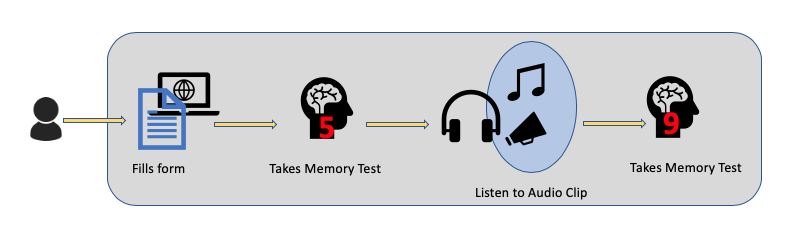
\includegraphics[width=\columnwidth]{images/ExptOverview.png}
    \caption{Experimental Design}
    \label{fig: Experiment}
\end{figure}

\noindent
For the memory exercise, we use an auditory implementation of the Digit Span game. With each game, a series of randomly generated digits from 0 to 9 are read out loud to the participant. The participant then has to recall the digits in the same order that they were read out. We start with a 2 digit number and kept increasing the sequence length by one (i.e. 3 digit, 4 digit etc.) each time the participant gives the correct answer. The game stops when the participant is unable to recall the sequence correctly. The game is designed to have every sequence be randomly generated each time it is played.

\subsection{Intervention}

The experiment is designed to have two groups: 1. A treatment group that receives calming audio and 2. A control group that receives loud stressful noises. We compiled the audio clips that we needed for our experiment using some freely available public audio clips on YouTube. Both clips played for a duration of 90 seconds each. The loud and stressful audio clip included a combination of noisy sounds like that of a siren, a crying baby, vehicles honking, an alarm clock ringing etc. The calming audio included the white noise of rainfall combined with a soft and soothing Zen music playing in the background. The audio clips were designed to induce a calming or stressful effect on the mind as the case may be. \\

\noindent
To ensure that were not introducing two opposing treatments using the aforesaid method, we made sure both the audio clips started with a small amount of the same common stressful noises for the same short duration before we transitioned into calm music versus loud and noisy sounds for the rest of the clip duration. We also ensured that we blanked out any video in the YouTube clip to keep it strictly as an audio clip and not introduce any sort distraction to the participants while providing the intervention.

\subsection{Survey Implementation and Hosting}

The setup for this experiment is minimalist for a face to face delivery mechanism. However, since this option was out of question for us, we had to look at an online delivery mechanism for the same. Online delivery for this type of survey which involves implementation of a memory game was neither easy nor straight forward using the popular survey infrastructures that we had access to. We therefore had to come up with a custom solution with our very own web survey HTML page and render it from a custom web service hosted on google cloud. Behind the scenes we linked the fields in the custom HTML form to a google form so that we could leverage the google form infrastructure to record and access participant responses. Google form responses are saved in a Google spreadsheet which we download for our data analysis. Figure \ref {fig: Survey} below shows the custom solution we used to host, render and record our survey via Google cloud.

\begin{figure}[h]
    \centering
    \includegraphics[width=\columnwidth]{images/Survey.png}
    \caption{Survey Hosting and Recording}
    \label{fig: Survey}
\end{figure}

\subsection{Measurement Strategy}

Considering the study in the light of our hypotheses, we were interested in measuring the pre-treatment and post-treatment scores of every participant. We were also interested in collecting data about participants on: 1. their gender 2. whether they received some form of music training (values ranged from no training to over 5 years of music training) 3. time of day when they took the survey. Since our participant were spread across different countries and geographies we asked them to choose from a bunch of local time ranges. We made all these fields mandatory in our survey page so that a participant would not be able to submit an incomplete form. Since we primarily relied on our friends and family to participate, we chose to record participant name so that we could reach out to them in case of missing responses. 

\subsection{Enrollment and Communication Strategy}

We did not require any special enrollment to participate in our survey. We used both personal emails and social media postings to request participation in our survey. In our communication we indicated clearly what the experiment was about and what was required to participate without revealing the design. We also used the Berkeley Announcement Channel on Slack to solicit participation. Appendix A gives a snapshot of the communication message we used to encourage participation. We followed this up with repeated reminders where possible to ensure we as many responses as we could gather. 

\subsection{Randomization}

Memory span and working memory is said to improve with age, peak at adulthood and gradually decline after adulthood. It therefore made sense to employ a randomized block design by dividing our subjects into blocks by age and do a randomized assignment within the blocks to control and treatment groups. This randomized block design would help reduce the noise that might be caused by age on the effect of our treatment and give us better precision on our outcome variable.  We used blocks of three age groups: 5 to 21 years, 21 to 55 years and above 55 years. We designed our survey to be accessible to anybody with a link to it. So it was important that we did the block randomization by age at the web server level using a persisted and centralized store. 

\subsection{Outcome Variable}

We analyze the data using 2 outcome variables of interest: 1. a dummy variable called \textit{score-improved} which indicates if a participant's score improved or not post treatment. 2. a difference in scores called \textit{score-difference} between pre-treatment and post-treatment scores. Our independent variable is \textit{treatment} which is a dummy for whether treatment in the form of calming audio was administered or not. Our covariates include \textit{pre-treatment score} which acts as baseline,  \textit{music}, \textit{gender} and \textit{time of day} as control variables.

\section{Data}  

We received a total of 148 complete responses. A closer inspection of the data showed us that 8 of these were duplicated\footnote {Duplicate response issue on google form and iOS, https://support.google.com/docs/thread/40862184?hl=en}. Eliminating these duplicates landed us with 138 unique responses. Of these, 65 were from those assigned to the control group and 73 from those assigned to the treatment group. It appears that 7 to 8 participants that were assigned to the control group attrited from the study. Our experiment randomized based on age blocks. We found 15 participants each assigned to treatment and control groups among ages 5 to 21. Of the complete responses, treatment assignment was 51.8\% in the age group 22 to 55 years and 60\% in the age group older than 55. We cover a more detailed analysis on the attrition observed in this experiment in section \ref{Attrition}. Table \ref{table: numbers} gives the distribution of participants by the assignment group.\\

\begin{table}[h]
\begin{center}
 \begin{tabular}{||c | c c ||} 
 \hline
 Participant Characteristic & Treatment & Control \\  
 \hline\hline
 Total count & 73 & 65 \\ \hline
 Age (5 - 21 years) & 15 & 15 \\ 
 Age(22 - 55 years) & 43 & 40^* \\ 
 Age(> 55 years) & 15 & 10^* \\ \hline
 Male & 32 & 24 \\ 
 Female & 33 & 49 \\ \hline
 Music training & 19 & 20 \\ 
 No music training & 27 & 25 \\ 
 & & \textit{* attrition observed} \\ \hline
 \end{tabular}
\caption{Participant numbers by Treatment}
\label{table: numbers}
\end{center}
\end{table}

\noindent
Figure \ref{fig: Histogram} shows the distribution of the scores from the memory tests and also the difference between them. The histogram for the post treatment score shows a shift in the mean scores to the right for both groups. However, the shift is more pronounced for the treatment group as evidenced in the histogram of score differences where the treatment group shows more positive difference than the control group. This gives us an indication that the treatment has a positive effect on the memory recall score. According to Miller's law\footnote {named after the celebrated cognitive psychologist George A Miller from Harvard University}, the human brain can remember and hold on to seven $\pm$ 2 objects on average \footnote {"The Magical Number Seven, Plus or Minus Two: Some Limits on Our Capacity for Processing Information", https://en.wikipedia.org/wiki/The\_Magical\_Number\_Seven,\_Plus\_or\_Minus\_Two}. While the mean scores of participants were well within this range for both tests, there were a couple of outliers. It is plausible that a couple of participants relied on external aids to help with their memory recall.  We don't correct for these outliers as they are random occurrences and are equally likely in treatment and control groups. \\

\begin{figure}[h]
    \centering
    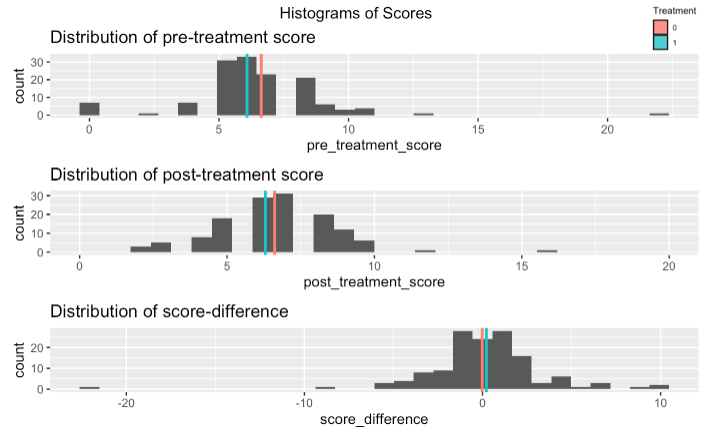
\includegraphics[width=\columnwidth]{images/Histogram.png}
    \caption{Distribution of Scores}
    \label{fig: Histogram}
\end{figure}

\begin{table}[h]
\begin{center}
 \begin{tabular}{||c c c c||} 
 \hline
 Treatment & pre-treatment-score & post-treatment-score	& score-difference \\  
 \hline\hline
 0 & 6.631 & 6.615 & -0.015 \\ \hline
 1 & 6.082 & 6.301 & 0.219 \\ \hline
\end{tabular}
\caption{Average Scores by Treatment}
\label{table: meanscores}
\end{center}
\end{table}

\noindent
Table \ref{table: meanscores} shows the average scores between the treatment and control groups. Figure \ref{fig: ScoreDiff} shows the box plots of the score differences for all the participants in the experiment and by the three age blocks. The variance in the treatment group is much smaller compared to the variance in the control group in the experiment overall as well as most age blocks. The score difference is marginally higher in the treatment groups for age blocks 5 to 21 years and older than 55 years. The difference in difference for the age block 22 - 55 years is not discernible. 

\begin{figure}[h]
    \centering
    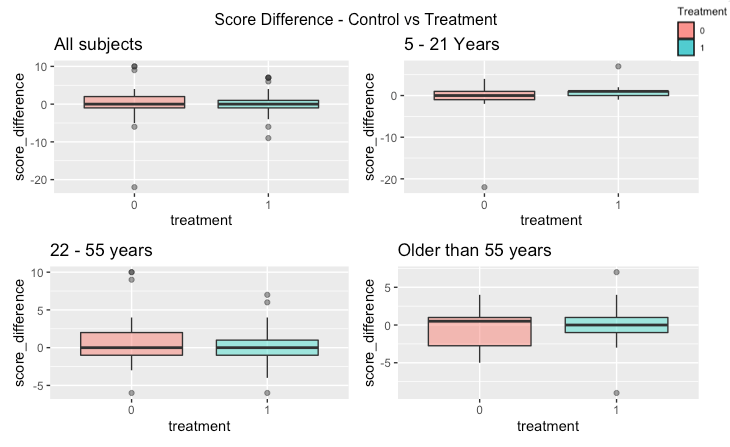
\includegraphics[width=\columnwidth]{images/ScoreDiff2.png}
    \caption{Survey: Box Plots of Score Differences}
    \label{fig: ScoreDiff}
\end{figure}

\section {Results}

\subsection {Validation}

Before looking at treatment effects and impact of covariates on the outcome variable, we first run validation checks on our data to ensure any regression analysis will give with unbiased estimates.

\subsubsection {Placebo Test}

A placebo test would tell us if we see a treatment effect when we are not supposed to see one. To validate this we regress the \textit{pre-treatment-score} on the treatment variable and other covariates. Since pre-treatment-score is computed before the treatment was meted out, we should not observe any statistically significant results for any of the covariates. 

\begin{table}[h]
    \centering
    \includegraphics[scale = 0.60]{images/PlaceboTest.png}
    \caption{Placebo Test: Coef-test on covariates}
    \label{fig: Placebo}
\end{table}

\noindent
From figure \ref{fig: Placebo}, we see that the p-value is not statistically significant for any of the covariates and the coefficients we see are just a chance occurrence.

\subsubsection {Covariate Balance Check}

To verify if the covariates balance out, we regress the treatment variable on all covariates of interest in our experiment. Figure \ref{fig: CovBal} shows the results of the covariate balance check. We can see that the check fails on two covariates: \textit{genderMale} and \textit{(Intercept)} which represents women who are in the age group 22- 55 years and who have had 1 to 2 years of music training. The distribution of the composition of \textit{(Intercept)} is given in table \ref{table: intercept}. One contributing factor to the imbalance could be the attrition we observe. 

\begin{table}[h]
    \centering
    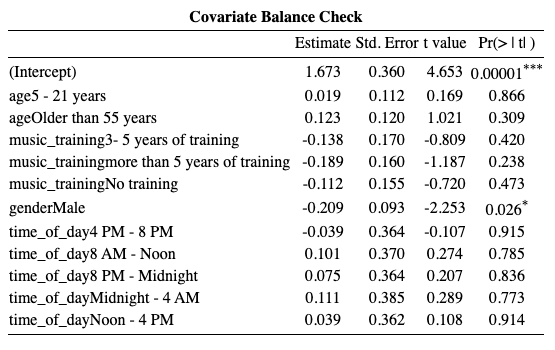
\includegraphics[scale = 0.6]{images/CovBal.png}
    \caption{Covariate Balance Check}
    \label{fig: CovBal}
\end{table}

\begin{table}[h]
\begin{center}
 \begin{tabular}{||c| c c||} 
 \hline
 Distribution & Treatment & Control \\  
 \hline\hline
 Women in Age (22 - 55 years) & 32 & 21 \\ \hline
 Women in Age (22 - 55 years) with 1-2 years of music training & 4 & 4 \\ \hline
 Men in Age (22 - 55 years) & 9 & 11 \\ \hline
\end{tabular}
\caption{Distribution of Intercept}
\label{table: intercept}
\end{center}
\end{table}

\noindent
From table \ref{table: intercept} we can see that the distribution of the intercept is not balanced between treatment and control groups because of the uneven distribution of women in age group 22 - 55 years. Similarly there are more men in the control group in the same age group. To get the ideal balance between the treatment and control groups, we would have had to do block randomization for every category of every covariate we have in the experiment making the experimental design very complex and the randomization quite difficult to handle. In our experimental design, we chose not block on gender because: (1) we do not believe that memory recall would be impacted by gender (2) we hoped that the random assignment would automatically take care of this. But we ended up with a chance uneven distribution of men and women in the experiment overall and in the age group 22 - 55 years. We will not use gender as a covariate in our regression analysis due to the imbalance we observe with this covariate. \\

\noindent
Additionally, we use a CRAN package called MatchIt\footnote{https://cran.r-project.org/web/packages/MatchIt/MatchIt.pdf} to preprocess the data and perform a covariate balance on it using the cobalt\footnote {Matching was performed using the Matching package (Sekhon, 2011), and covariate balance was assessed using cobalt (Greifer, 2020), both in R (R Core Team, 2020).} package. MatchIt is designed for causal inference and tries to create covariate balance by selecting, duplicating or selectively dropping observations without inducing bias. The balanced abd adjusted data given by MatchIt has 130 complete responses. Appendix \ref{appendix:C} shows the balance plots on the data. 

\begin{figure}[h]
    \centering
    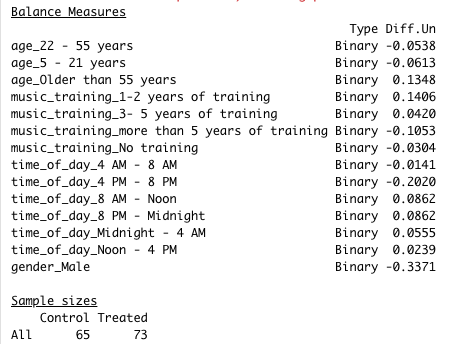
\includegraphics[scale=0.6]{images/Cobalt.png}
    \caption{Covariate Balance performed with MatchIt}
    \label{fig: cobalt}
\end{figure}

\noindent
We will do comparative analysis of our outcome variables both using both the raw original data  as well as the covariate balanced data given by the MatchIt package. We will add gender to our models when using the matched data only.

\subsection {Analysis}
We also believe that there may be some correlation between stress levels and time of the day. For example stress levels may be potentially higher at work hours than off work hours.

\subsubsection{Score Improvement Dummy as Outcome}

We first analyze the treatment using an indicator variable called \textit{score-improved} which is set to 1 if the memory recall score does not decrease post treatment or 0 if otherwise. The tally of the score improvement and the mean outcomes among compliers is tabulated in table \ref{table: scoreimp}. We see a local average treatment effect (CACE or LATE) of 0.104.

\begin{table}[h]
\begin{center}
 \begin{tabular}{||c| c c||} 
 \hline
 Effect & Treatment & Control \\  
 \hline\hline
 Participants for whom score improved & 48 & 25 \\ \hline
 Participants for whom score deteriorated & 36 & 29 \\ \hline
 Mean Outcome & 0.658 & 0.554 \\ \hline
 \end{tabular}
\caption{Tally - Score Improvement}
\label{table: scoreimp}
\end{center}
\end{table}

\subsubsection*{Short Model}\\
We run a simplistic model of regressing the outcome variable with the treatment variable and do this on all three of our age blocks to estimate the effect of our treatment on score improvement.

\begin{table}[h]
    \centering
    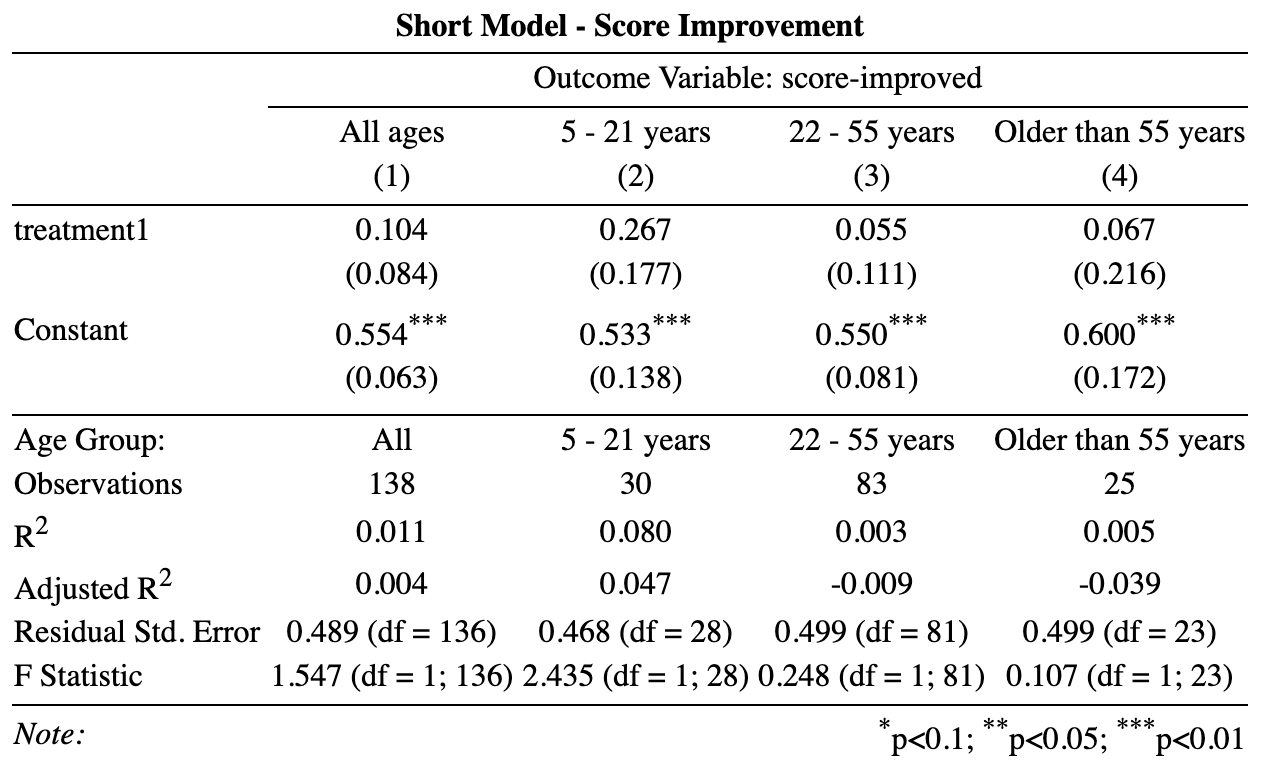
\includegraphics[scale = 0.6]{images/score-imp1.png}
    \caption{Short Model - Score Improvement}
    \label{fig: scoreimp1}
\end{table}

\noindent
Table \ref{fig: scoreimp1} shows a positive treatment effect of 0.104 which indicates that for every person who received the treatment there was a 10.4 percent increase in  score improvement and this improvement is seen across as three age groups. We see a 26.7 percent increase in the age group 5 - 21 years, a 5.5 percent increase in the age group 22 - 55 years and a 6.7 percent increase in the age group above 55 years. However, the p-values of these effects are not statistically significant. The $R^2$ value of this model is quite low indicating that the model is unable to explain much of the variance in the outcome variable. So we look into adding more covariates to see if we can explain some of this variance observed in the treatment effects.

\begin{table}[!t]
    \centering
    \includegraphics[width=\columnwidth]{images/scoreimp3A.png}
    \caption{Long Model with Matched Data - Score Improvement}
    \label{table: scoreimp3}
\end{table}

\subsubsection*{Long Model with Balanced Data} \label{longModel2}
We use the data balanced by MatchIt to analyze the impact of treatment on score improvement. We believe that a calming audio treatment might have different impacts at different times of the day. So we interested in the heterogenous treatment effects of treatment on time of day. We are alos curious to see if men and women react differently to treatment. Table \ref{table: scoreimp3} summarizes the results of this long model. 
The $R^2$ values of this long model is higher than that of the short model, indicating that the long model is able to explain much more of the variance seen in the treatment variable. The F statistics is significant indicating that the long model is better at explaining the effects of the covariates on the outcome variable. \\

\noindent
Treatment has a positive effect on score improvement among youngsters and adults in this sample. Men perform similar to women in the young and adult groups. However, men show slightly improved scores compared to women in the senior age group (i.e. older than 55 years). We see that music has a statistically significant positive effect of 33.8\% on score improvement among youngsters. 8PM to midnight has a statistically significant unfavourable impact on score improvement among adults in the age group 22-55 years. This could possibly be because our body is exhausted both physically and mentally by the end of the day and therefore might not be an ideal time to take a memory test. Similarly noon to 4PM has a statistically significant negative effect of 72.5\% on score improvement and youngsters. The treatment had a statistically significant negative impact on young men/boys. Young boys that were given the audio treatment showed a negative effect of 71.1\% on score improvement. \\

\noindent
While we are unable to see statistically significant effects of treatment to imply causation in general, we do see that the treatment has a negative causal impact among young men in age 5 - 21 years. The calming audio treatment does show a positive impact on score improvement at all times of the day. But we don't see any statistically significant p-values to assert causation. 

\subsubsection{Score Difference as Outcome}

To get a better understanding of how much score difference we see between the treatment and control groups as an effect of the audio treatment, we regress the \textit{score-difference} outcome variable on our treatment variable and covariates of interest.

\subsubsection*{Score Difference - Short Model}
We first look at a short model that regresses \textit{score-difference} on the treatment variable. Table \ref{table: scorediff1} summarizes the regression results. There is a positive treatment effect of 0.235 on the score difference which says that people who were exposed to the calming audio treatment saw a score increase of 23.5 \% on an average. However, this result is not statistically significant to suggest causation.

\begin{table}[!h]
    \centering
    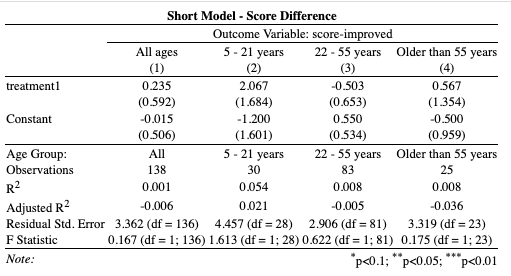
\includegraphics[scale = 0.7]{images/score_diff1.png}
    \caption{Short Model - Score Difference}
    \label{table: scorediff1}
\end{table}

\subsubsection*{Long Model with Matched Data}\\

We now look at the long model on the matched data using the same covaritaes as we used in section \ref{longModel2}. From the regression summary in table \ref{table: scorediff3} we can see that the model gives an over positive treatment effect. Music has a positive impact on memory recall only among youngsters. 8 PM to midnight seems particularly unsuitable for memory tests with a negative effect of -1.191. However, participants who were given the calming audio treatment at this time saw a positive effect of 1.556 on their score difference. \\

\noindent
In general the calming audio treatment had a positive effect on score differences on most times of the day as we can see that the coefficients for most of these jumped from negative effect to positive in the presence of audio treatment. Treatment seemed to have a negative impact from midnight to 8AM. It is plausible that listening to audio clip at an already quiet and calm time of the night, has a counter effect on the mind and affects the ability to recall effectively. None of the observations related to treatment or its interaction terms seem to have a statistically significant value to suggest a causal impact.

\begin{table}[h]
    \centering
    \includegraphics[scale = 0.7]{images/score_diff3.png}
    \caption{Long Model with Matched Data - Score Difference}
    \label{table: scorediff3}
\end{table}

\subsection {Power}

Power depends on treatment effect, variance and sample size. With a sample size of 138, we were only able to achieve a power of 23.6\% and 7.1\% for outcome variables \textit{score-improved} and \textit{score-difference} respectively. To increase the power to 80\% with the same sample size, we would need to either reduce our sample variance or increase the local treatment effect as show in figure \ref{fig: power1} for \textit{score-improved} and in figure \ref{fig: power2} for \textit{score-difference}.
\begin{figure}[h]
    \centering
    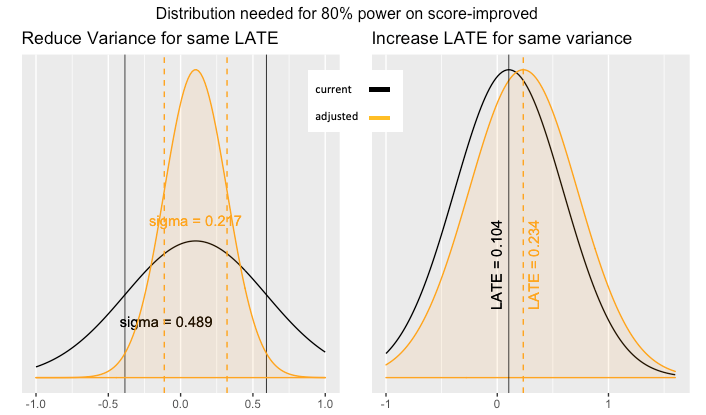
\includegraphics[scale=0.6]{images/power1.png} 
    \caption{Power adjustments for score-improved}
    \label{fig: power1}
\end{figure}
    
\begin{figure}[!h]
    \centering
    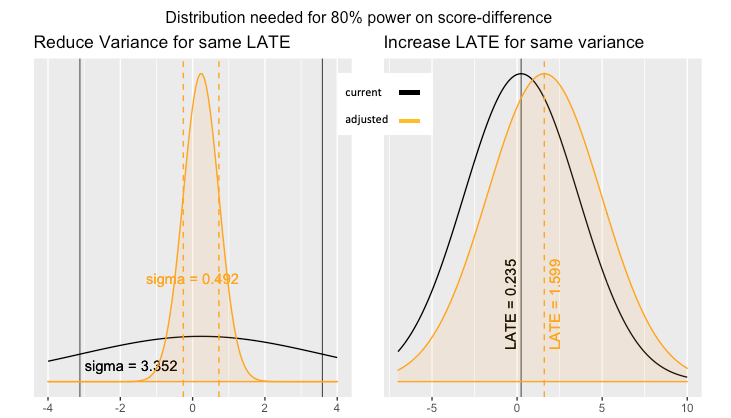
\includegraphics[scale=0.6]{images/power2.png}
    \caption{Power adjustments for score-difference}
    \label{fig: power2}
\end{figure}

\noindent
The same treatment effect and variance, we would need a much larger sample size to get an experiment with 80\% power. Table \ref{table: power3} gives an idea of how big a sample size we would need to get 80\% power out of our experiment for the same treatment effect and variance

\begin{table}[h]
\begin{center}
 \begin{tabular}{||c| c c c||} 
 \hline
 Outcome Variable & LATE & Sigma & Sample Size \\  
 \hline\hline
 score-improved & 0.104 & 0.489 & 175 \\ \hline
 score-difference & 0.235 & 3.352 & 1603 \\ \hline
 \end{tabular}
\caption{Sample Size Required for 80\% Power}
\label{table: power3}
\end{center}
\end{table}

\subsection {Attrition} \label{Attrition}
Based on the number of responses we see in each age block for the treatment and control groups, we know that they has been some level of attrition. We find 7 to 8 missing records indicating that we have and overall attrition of 5.5 percent. The attrition seems to be systemic to the control group as we see that all missing records belong to the control group. The differential attrition caused by treatment is 8.75 to 9.88 percent. The control group in our experiment received an audio treatment in the form of loud and stressful noises. It is possible that some of the participants in the experiment found the noise unpleasant and stressful and quit the experiment midway.


\section {Conclusion}

In this study we designed an experiment to answer the research question: does a relaxed mind cause one to remember information better? We designed an experiment based on difference in difference approach to help answer our research question. While we observed a positive treatment effect on memory recall, our experiment lacked enough powered to detect a statistically significant result. We hypothesised that significant music training and time of day have an impact on memory recall. We observed a statistically significant positive effect of more than 5 years of music training on improved memory recall among youngsters in ages 5 - 21 years. We also observed that taking the memory test between 8PM to midnight had a statistically significant negative impact on memory recall scores. We also observed that the treatment on young males in ages 5 - 21 had a negative impact on memory recall scores.

\subsection{Limitations}

We used an online experimental setup to gather the data required for our causation analysis and relied on our friends and family to respond to the experiment. We learnt very soon that it is not easy to come by responses quickly. \\

The exclusion restriction is hard to enforce in an online experimental setup. In our experiment the treatment was delivered in the form of an audio clip. Since we relied on friends and family to respond to the survey, in many cases there were more than one participants from the same household. We gave explicit instructions asking participants to wear headsets or be alone in a quite room. But there was no way to enforce this. We trust the participants followed the instructions correctly not violating the exclusion restriction. \\

While the treatment may have been effective, the treatment effects we observed were very small and the variance was quite high given us an under powered experiment. With an under powered experiment it is nearly impossible to find a statistically significant result that could lead to a causal implication. 

\subsection{Future Work}



\clearpage
\section{References}
\vspace*{3mm}
\begin{enumerate}
  \item Reference 1 , https://arxiv.org/pdf/1506.07285.pdf .
  
  \item Reference 2, https://www.aclweb.org/anthology/W18-2603.pdf.

  \item Reference 3, https://arxiv.org/pdf/1704.00051.pdf.
  
  \item
  @Article{,
    title = {{MatchIt}: Nonparametric Preprocessing for Parametric
      Causal Inference},
    author = {Daniel E. Ho and Kosuke Imai and Gary King and Elizabeth
      A. Stuart},
    journal = {Journal of Statistical Software},
    year = {2011},
    volume = {42},
    number = {8},
    pages = {1--28},
    url = {http://www.jstatsoft.org/v42/i08/},
  }


\end{enumerate}

% include your own bib file like this:
%\bibliographystyle{acl}
%\bibliography{acl2015}

%\begin{thebibliography}{}

%\bibitem[\protect\citename{Aho and Ullman}1972]{Aho:72}
%Alfred~V. Aho and Jeffrey~D. Ullman.
%\newblock 1972.
%\newblock {\em The Theory of Parsing, Translation and Compiling}, volume~1.
%\newblock Prentice-{Hall}, Englewood Cliffs, NJ.

%\end{thebibliography}

\clearpage
\appendix
\section{Appendix: Message to Participants }
\label{appendix:A}
\begin{enumerate}
 \item \large{Email Communication} 
\vspace*{+2mm}
\begin{figure}[h]
    \includegraphics[scale=0.62, left]{images/Model1_sample.png}
    \caption{Sample Predictions: Model-1 (baseline)}
    \label{fig: Model1_2}
\end{figure}
\end{enumerate}

\section{Appendix: Survey}
\label{appendix:B}
\begin{enumerate}
\item \large{Link to Survey}
\item \large{Web Service Code}
\vspace*{+2mm}
\begin{figure}[h]
    \includegraphics[scale=0.62, left]{images/Model1_sample.png}
    \caption{Sample Predictions: Model-1 (baseline)}
    \label{fig: Model1_2}
\end{figure}

\item \large{Survey Pages}
\vspace*{+2mm}
\begin{figure}[h]
    \includegraphics[scale=0.62, left]{images/Model1_sample.png}
    \caption{Sample Predictions: Model-1 (baseline)}
    \label{fig: Model1_2}
\end{figure}
\end{enumerate}

\clearpage
\section{Appendix: Additional Regression Analysis }
\label{appendix:C}
\subsubsection*{Long Model for Score Improvement with Raw Data}
Based on our hypothesis, we add the pre-treatment score, music training for those that have had over five years of music training and time of day as covariates to our regression model. We drop gender as we were unable to achieve covariate balance on gender. \\

\begin{table}[!b]
    \centering
    \includegraphics[width=\columnwidth]{images/scoreimp2A.png}
    \caption{Long Model - Score Improvement}
    \label{fig: scoreimp2}
\end{table}

\noindent
We observe that treatment still has a positive effect on age groups 5 to 21 years and 22 to 55 years in this sample. But its effects don't have any statistical significance to suggest a causal impact. 8PM to midnight has a statistically significant negative impact and seems to be a particularly bad time to take the memory test plausibly because our brains are more tired closer to the end of the day. Music has a statistically significant positive effect on memory recall among youngsters. Noon to 4PM has a statistically significant negative impact among youngsters in this sample. We cannot make any causal suggestions for covariates like music or time of day as we did not control from them in this study.

\clearpage
\section{Appendix: Additional Plots }
\label{appendix:D}
\begin{enumerate}
\item \large{Covariate Balance Plots on matched data using Cobalt and MatchIt packages}
%%\vspace*{+2mm}
\begin{figure}[h]
    \centering
    \begin{subfigure}{\textwidth}
    \includegraphics[width=\columnwidth]{images/balplot1.png} 
    \end{subfigure}
    \begin{subfigure}{\textwidth}
    \includegraphics[width=\columnwidth]{images/balplot2.png}
    \end{subfigure}
\vspace*{+5mm}
\caption{Cobalt balance plots showing the difference between unadjusted and adjusted data for each covariate}
\label{fig: balplot}
\end{figure}
\end{enumerate}

\clearpage

\end{document}